\section{Алгоритм анализа регулярных множеств}
Целью данной работы является создание алгоритма синтаксического анализа регулярных множеств, который может быть применим для анализа встроенных языков. Как упоминалось ранее, встроенный код порождается в момент выполнения основной программы. Для генерации могут использоваться строковые операторы, условные операторы и циклы из-за чего такой код не может быть представлен линейно. Результатом работы лексического анализатора на таком коде является не линейный поток токенов, а конечный автомат над алфавитом токенов. В рамках данной работы на такие автоматы накладывается следующее ограничение: они должны быть детерминированными. Если это условие не будет выполняться, то нельзя будет однозначно выбрать, по какому пути производить разбор. Например, для встроенного кода на листинге~\ref{lst:brExpr} будет построен конечный автомат на рис.~\ref{input}.

%\fvset{frame=lines,framesep=5pt}
\begin{listing}
\begin{pyglist}[language=csharp,numbers=left,numbersep=5pt]
 string expr = "" ;
 for(int i = 0; i < len; i++) 
 {
     expr = "()" + expr;
 }
\end{pyglist}
\caption{Код на C\#, динамически формирующий скобочную последовательность}
\label{lst:brExpr}
\end{listing}

\begin{figure}[h]
 \centering
 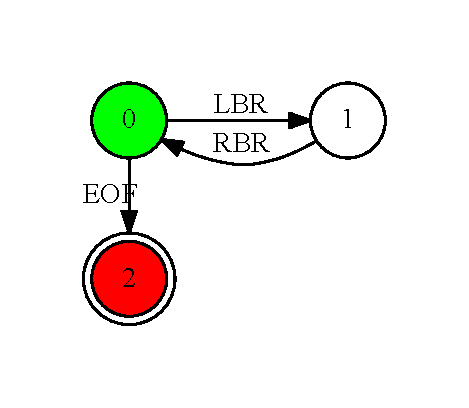
\includegraphics[width=0.3\textwidth]{Ragozina/pics/input.pdf}
 \caption{Конечный автомат, представляющий аппроксимацию встроенного кода для листинга~\ref{lst:brExpr} }
 \label{input}
\end{figure}

В алгоритме вместо хранения позиции во входном потоке теперь хранится номер вершины во входном графе. Поскольку вход является нелинейным, то вместо того, чтобы просматривать один текущий входной символ на каждом шаге, рассматриваются все исходящие рёбра для текущей вершины и выбирается одно (как упоминалось ранее, автомат детерминирован, поэтому это возможно), соответствующее текущему терминальному символу в грамматике. Если такого ребра нет, то алгоритм просто продолжает свою работу --- из очереди достаётся новый дескриптор и процесс возобновляется. 

Для автоматического создания синтаксических анализаторов существует несколько подходов. В рамках первого подхода весь код парсера генерируется по грамматике. Чаще всего такой подход используется при генерации анализаторов, построенных методом рекурсивного спуска. При генерации нисходящих анализаторов для каждого нетерминала генерируются функции, которые последовательно вызываются в процессе разбора. Несмотря на то, что нисходящие анализаторы просты для разработки, и поэтому чаще всего создаются вручную, существуют инструменты для автоматической генерации таких анализаторов. Например, инструмент ANTLR~\cite{antlr} --- генератор парсеров, позволяющий автоматически создавать анализаторы на одном из целевых языков программирования по описанию LL(*)-грамматики на языке, близком к EBNF. Структура генераторов такого типа изображена на рис.~\ref{genTypes}{\it (а)}.

\begin{figure}
 \centering
 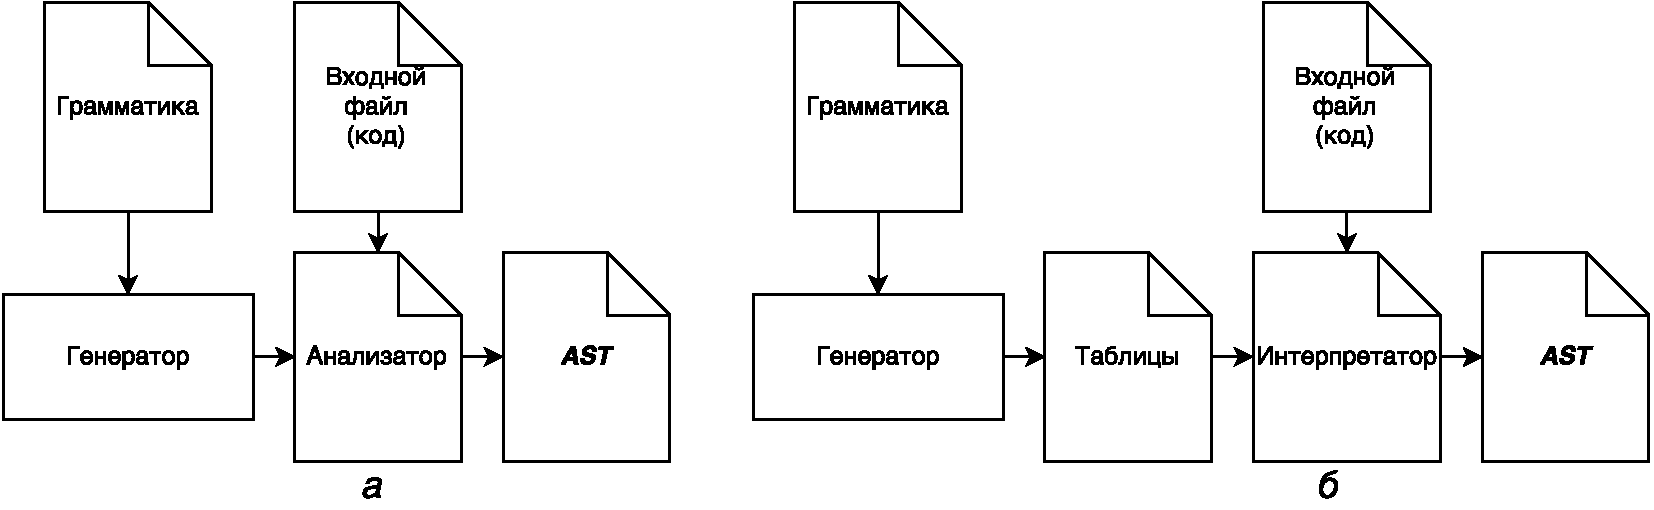
\includegraphics[width=\textwidth]{Ragozina/pics/GeneratorTypes.pdf}
 \caption{Подходы к генерации синтаксических анализаторов}
 \label{genTypes}
\end{figure}

Существует ещё один подход для генерации синтаксических анализаторов, который используется для получения табличных анализаторов. Отдельно создаётся интерпретатор, который содержит в себе основную логику алгоритма. Интерпретатор пишется вручную и переиспользуется. По грамматике каждый раз генерируется дополнительная информация, которая необходима интерпретатору в процессе работы. Структура такого генератора представлена на рис.~\ref{genTypes}{\it (б)}. Чаще всего в качестве дополнительной информации генерируются таблицы синтаксического анализа, управляющие процессом разбора.

В оригинальных работах, описывающих GLL-алгоритм, используется первый подход. В рамках данной работы был выбран второй подход из-за его гибкости и универсальности. Вместо генерации функций по слотам грамматики и их последовательного вызова, в главном цикле алгоритма просто рассматриваются все возможные состояния, в которых может находиться парсер. В зависимости от того, какой символ во входном потоке и какая позиция в грамматике, в процессе разбора рассматриваются следующие ситуации.

\begin{itemize}
\item Если текущий символ в грамматике является терминалом $x$ и существует исходящее из текущей вершины ребро, помеченное этим нетерминалом, то указатель в грамматике нужно сдвинуть на одну позицию вправо, $x \rightarrow \alpha X \cdot \beta$, и текущей вершиной назначить конечную вершину ребра. Никаких дополнительных действий со стеком при этом не производится. Иначе, если нет ребра, помеченного терминалом $х$, то текущая ветка разбора считается ошибочной, отбрасывается и  разбор продолжается с использованием следующего дескриптора.
\item Если текущий символ в грамматике является нетерминалом $a$, то необходимо в стек записать слот, по которому продолжить разбор после того, как правило для $a$ будет разобрано. Указатель в грамматике перемещается на $a \rightarrow \cdot \gamma $, а номер вершины во входном потоке остаётся без изменений.
\item Если указатель в грамматике имеет следующий вид $x \rightarrow \alpha\cdot$ и стек не пуст, то слот вида $y \rightarrow \delta x \cdot \mu$, который хранится в этот момент в текущей вершине стека, извлекается и становится текущим.
\item Если текущий слот имеет вид $s \rightarrow \tau\cdot$, и весь входной поток рассмотрен, то разбор завершается успешно, иначе разбор заканчивается ошибкой. В случае успешного завершения разбора возвращается дерево, иначе сообщение об ошибке.
\end{itemize}

Наличие циклов во входном графе никак не влияет на процесс разбора. Дескрипторы позволяют без каких-либо изменений процесса разбора обработать их. Это делает результирующий алгоритм более простым в отличие от алгоритма, основанного на RNGLR , в который потребовалось внести существенные изменения для поддержки циклов~\cite{RelaxedARNGLR}. За счёт того, что каждый раз при добавлении дескриптора выполняется проверка всей четвёрки целиком (позиция во входе, слот, вершина стека и часть леса разбора), то лишние дескрипторы с одинаковыми деревьями не создаются. Переиспользование уже созданных узлов также позволяет избежать создания лишних деревьев: если дерево с определёнными координатами и соответствующим правилом вывода уже было создано, то повторно такое дерево создаваться не будет.

В алгоритме так же поддерживается четвёрка: слот (вместо имени функции), номер вершины в графе, вершина стека и узел дерева. Поскольку вызов функций заменён на обработку ситуаций, возникающих в процессе анализа, в теле основной функции, то появилась необходимость определять, какое правило вывода использовать для разбора. Для определения правила используются LL-таблицы, где в каждой ячейке может быть несколько правил для разбора, что соответствует ситуации наличия в грамматике неоднозначностей. Анализатор состоит из функции, содержащей основной цикл алгоритма, функции управляющей процессом разбора и функций для построения дерева и стека.

\begin{listing}[H]
\hrule
\begin{algorithmic}
\caption{Функция, содержащая в себе основную логику алгоритма}
\label{parsing}
\Function{parsing()}{}
	\State{$condition \gets true$}
	\If{$isEpsilonRule(cL.rule)$} 
		\State{$cR \gets$ $new TerminalNode("Epsilon", packExtension (cI, cI))$}
		\State{$cN \gets$ $getNodeP(cL, cN, cR)$}
		\State{$pop(cU, cI, cN)$}
    \Else
		\If{$isEndOfRule(cL.rule, cL.position)$}
			\State{$curSmb \gets$ $grammarRules[cL.rule][cL.position]$}
			\If{$isTerminal(curSmb)$}
				\State{$curSmb \gets$ $grammarRules[cL.rule][cL.position]$}
				\If{$cI.OutEdges$ contains edge labeled with $curSmb$}
					\State{$curEdge \gets$ edge labeled with $curSmb$}
					\State{$cR \gets$ $getNodeT(curEdge)$}
					\State{$cI \gets$ $curEdge.TargetVertex$}
					\State{$cL \gets$ $label(cL.rule, cL.position + 1)$}
					\State{$cN \gets$ $getNodeP(cL, cN, cR)$}
				    \State{$condition \gets$ $false$}
				\EndIf
			\Else
				\State{$cU \gets$ $create(cI, label(cL.rule, cL.position + 1), cU, cN)$}
				\ForAll{$edge$ in outgoing edges of $cI$}
					\ForAll{$rule in table[curSymbol, edge.Token]$}
						\State{$addContext(cI, packLabel(rule, 0), cU, \$)$}
					\EndFor
				\EndFor	
			\EndIf
		\Else
		    \State{$pop(cU, cI, cN)$}
		\EndIf
    \EndIf
\EndFunction
\end{algorithmic}

\hrule
\end{listing}

\begin{listing}
\hrule
\begin{algorithmic}
\caption{Функции, управляющие процессом разбора }
\label{control}
\Function{control()}{}
	\State{$condition \gets$ $true$}
	\While{not $stopr$}
		\If{$condition$} {$dispatcher()$}
		\Else {$processing()$} 
		\EndIf
	\EndWhile
\EndFunction

\Function{dispatcher()}{}
	\If{$\mathcal{Q}$ is not empty} 
		\State{$currentContext \gets$ $\mathcal{R}.Dequeue()$}
		\State{$cI \gets$ $currentContext.Index$}
		\State{$cU \gets$ $currentContext.GSSNode$}
		\State{$cL \gets$ $currentContext.Label$}
		\State{$cN \gets$ $currentContext.SPPFNode$}
		\State{$cR \gets$ $DummySPPFNode$}
		\State{$condition \gets$ $false$}
    \Else
		\State{$stop \gets$ $true$}
    \EndIf
\EndFunction
\end{algorithmic}
\hrule
\end{listing}

На листинге~\ref{control} приведены две функции управляющие разбором. Функция \texttt{control()} в зависимости от значений булевых переменных \texttt{stop} и \texttt{condition} вызывает функции \texttt{dispatcher()} или \texttt{parsing()}. Функция \texttt{dispatcher()} извлекает из очереди дескриптор, присваивает значения переменным. Функция \texttt{parsing()} на листинге~\ref{parsing} содержит в себе основную логику алгоритма.


\subsection{Пример работы алгоритма}
Рассмотрим следующий пример. В качестве входных данных будем испоьзовать конечный автомат $M$, представленный на рис.~\ref{InputGraph}, который генерирует произвольные скобочные последовательности. Необходимо построить лес разбора для всех цепочек, порождаемых автоматом $M$, выводимых в грамматике $G_4$ (листинг~\ref{grmG4}), описывающей язык правильных скобочных последовательностей.
\begin{listing}
\caption{Грамматика $G_4$}
\label{grmG4}
\centering
$\begin{array}{rl}
s \rightarrow LBR \ s \ RBR \ s \ \varepsilon \  | \ \varepsilon 
\end{array}$
\end{listing}

\begin{figure}
 \centering
 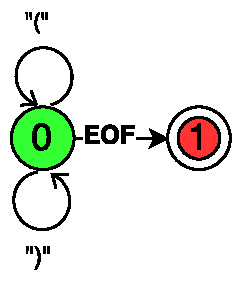
\includegraphics[width=0.3\textwidth]{Ragozina/pics/ExampleInputGraph.pdf}
 \caption{Конечный автомат, подаваемый на вход анализатору }
 \label{InputGraph}
\end{figure}

В результате работы описанного алгоритма построено сжатое представление леса разбора, представленное на рис.~\ref{ExSppf}. Циклы в сжатом представлении леса разбора отображают наличие циклов во входном конечном автомате и позволяют извлекать потенциально бесконечное множество деревьев, каждое из которых соответствует цепочке, порождаемой автоматом.

\begin{figure}
 \centering
 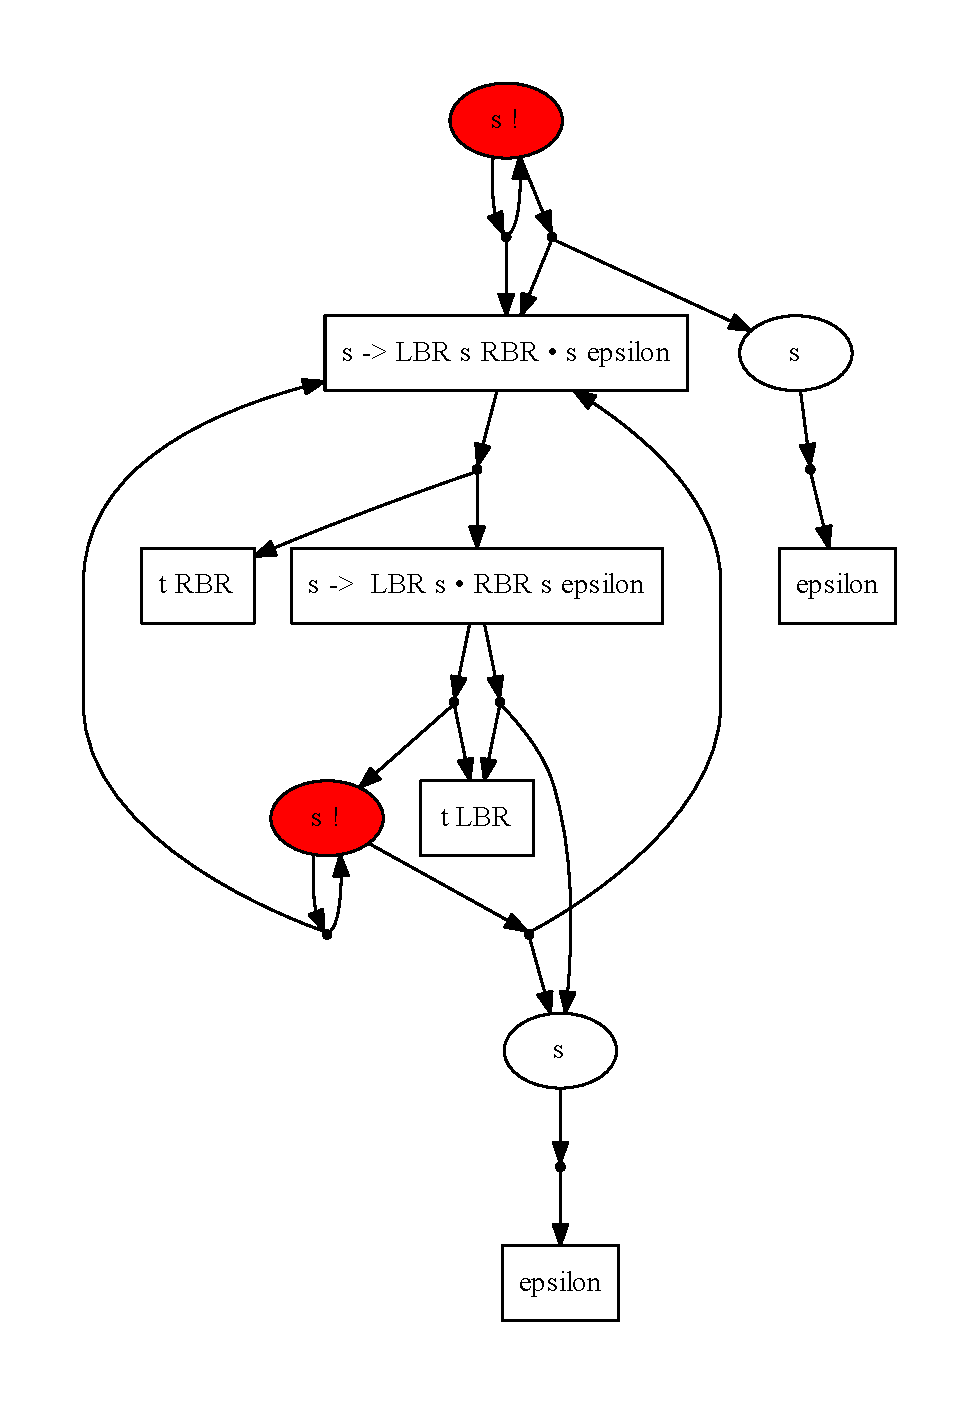
\includegraphics[width=\textwidth]{Ragozina/pics/SppfExample.pdf}
 \caption{Сжатое представление леса разбора для грамматики $G_4$ и конечного автомата на рис.~\ref{InputGraph} }
 \label{ExSppf}
\end{figure}

\subsection{Доказательство корректности}
Для того чтобы показать, что предложенный алгоритм работает корректно сначала нужно доказать, что процесс останавливается.

\textsc{Теорема 1.} 
\textit{Алгоритм завершает свою работу для произвольного детерминированного конечного автомата и контекстно-свободной грамматики.}

\textsc{Доказательство.}

Алгоритм завершает свою работу как только очередь дескрипторов становится пустой. Дескриптор с определённым набором значений полей в очередь добавляется лишь единожды. Таким образом, чтобы показать завершаемость алгоритма достаточно доказать, что количество дескрипторов конечно. 

Дескриптор состоит из четырёх элементов --- слот, индекс во входном потоке, вершина стека, дерево. Таким образом, общее количество дескрипторов не превышает прямого произведения возможного количества каждого из этих элементов. Количество индексов не больше количества вершин входного графа. Количество слотов конечно, потому что грамматика конечна. Вершина стека определяется парой --- слот и индекс, и значит тоже конечно. Часть леса, хранимая в дескрипторе, определяется однозначно именем нетерминала или слотом и двумя координатами во входном графе. Обе составляющие конечны. $\square$

Таким образом было показано, что количество дескрипторов --- конечное число.

\textsc{Определение 1.} 
\emph{Корректное дерево}~--- это упорядоченное дерево со следующими свойствами.
\begin{enumerate}
  \item Корень дерева соответствует стартовому нетерминалу грамматики $G$.
  \item Листья соответствуют терминалам грамматики $G$. Упорядоченная последовательность листьев соответствует некоторому пути во входном графе.
  \item Внутренние узлы соответствуют нетерминалам грамматики $G$. Потомки внутреннего узла (для нетерминала $N$) соответствуют символам правой части некоторой продукции для $N$ в грамматике $G$.
\end{enumerate}

Для того, чтобы доказать, что SPPF содержит только корректные деревья, сначала необходимо доказать следующую лемму.

\textsc{Лемма 1.} 
\textit{Для любой части леса $t$, построенного в процессе вывода, существует путь в графе $р$, такой что крона $t$ покрывает этот путь. }

\textsc{Доказательство.}

Для доказательство используется индукция по построению SPPF. 

\textsc{База.}

Для терминальных узлов утверждение очевидно. Терминальный узел соответствует ровно одному ребру во входном графе и строится только после прохода по этому ребру. Построение эпсилон узлов никак не зависит от входного графа, а производится только в соответствии с грамматикой. 

\textsc{Переход.}

Достаточно доказать для упакованных ячеек, всё остальное доказывается аналогично. Создание упакованных ячеек происходит в двух случаях --- при чтении нового терминала из входного потока или изъятии вершины стека, что значит, что текущий нетерминал был разобран и необходимо вернуться к точке, с которой этот разбор начался. 

Рассмотрим первый случай. У нас есть часть леса, которая соответствует какому-то пути $p$ в графе от вершины $v_0$ до $v_1$. Текущая позиция во входном потоке соответствует правой координате для этой части SPPF. При считывании нового терминала, создаётся упакованная ячейка, левым сыном которой становится уже построенная часть SPPF, а правым --- терминал. Получаем новую часть леса, соответствующее пути $P_1 = v_0 \dots v_1 v_{1+1}$.

Рассмотрим второй случай --- изъятие вершины со стека. Первая часть леса разбора Т1 хранится на ребре стека. Вторая часть Т2 построена по только что разобранному правилу. Каждая из этих частей соответствует какому-то подпути в графе и необходимо показать, что правая координата T1 совпадает с левой координатой T2. Это соответствует тому факту, что объединение этих частей леса даст часть леса, покрывающую путь в графе без дыр, то есть если в графе была цепочка {\it ``abcd''} и T1 соответствует {\it ``ab''}, то T2 будет соответствовать {\it ``bc''}. Для того, чтобы показать, что это условие выполняется, достаточно рассмотреть, как происходит процесс разбора. Как только в процессе обхода грамматики (в слоте) встречается нетерминал, создаётся новая вершина стека, которая хранит в себе слот с позицией за этим нетерминалом, на ребре хранится уже построенная часть леса. Правая координата этой части SPPF является номером вершины, с которой будет происходить дальнейший разбор, это число и записывается в новый дескриптор. Таким образом, после того, как нетерминал будет разобран до конца, будет создан новый упакованный узел, в котором в качестве левого потомка будет часть леса с ребра, а в качестве правого --- нетерминальный узел, левая координата которого совпадает с правой координатой левой части леса, так как именно с того места и начался разбор этого нетерминала. $\square$

Таким образом для упакованных узлов в дереве доказали необходимое. Доказательство для остальных видов узлов проводится аналогично.

\textsc{Теорема 2.} 
\textit{Любое дерево, извлечённое из SPPF, является корректным.}

\textsc{Доказательство.}

Рассмотрим произвольное извлечённое из SPPF дерево и докажем, что оно удовлетворяет определению. Первый и третий пункт определения корректного дерева следует из определения SPPF. 

Второй пункт следует из Леммы 1. Необходимо только показать, что такой путь начинается в начальной вершине и заканчивается в конечной. Действительно, так как работа алгоритма может быть начата только из начальной вершины, то левой координатой для неё будет стартовая вершина. Результатом работы алгоритма является SPPF. Узел помечается, как результирующий, если он помечен стартовым нетерминалом и его левая координата является стартовой вершиной, а правая --- финальной. $\square$

\textsc{Теорема 3.} 
\textit{Пусть грамматика Г порождает язык $L$. Тогда для каждого пути в графе $p$, соответствующего строке s из $L$, из SPPF может быть изъято корректное дерево.}

\textsc{Доказательство.}

Необходимо доказать, что SPPF содержит все корректные деревья вывода для всех корректных цепочек из входа. Как только процесс разбора начинается, в очередь дескрипторов добавляются дескрипторы для всех альтернатив стартового правила, соответствующие терминалу во входном потоке. Аналогичная ситуация происходит, как только в грамматике встречается нетерминал. Рассматриваются все альтернативы нетерминала и добавляются те, по которым может быть продолжен синтаксический анализ в соответствии со входным символом. Это гарантирует, что все альтернативы в выводе будут рассмотрены. При этом во входном графе все пути, соответствующие входным цепочкам, тоже рассматриваются, так как переход по ребру осуществляется всегда, если оно продолжает корректный префикс.$\square$

\subsection{Анализ данных большого объёма}
Одной из задач, сформулированных в данной работе, является использование предложенного алгоритма для анализа больших данных. Это востребовано, например, в задачах биоинформатики. Прежде чем формулировать задачу, следует ввести основные определения.

Исследование геномов является одной из распространённых задач биоинформатики. Информацию, содержащуюся в геноме можно представить в виде последовательностей символов и в дальнейшем эти последовательности анализировать. Геномы извлекаются из ДНК и позволяют характеризовать тот или иной организм. Для этого из генома необходимо выделить определённые участки, позволяющие сделать выводы о его свойствах. Геном (последовательность ДНК) --- строка в алфавите $\{A, C, G, T\}$, однозначно определяющая организм (или штамм), к которому она относится. Сборка --- набор подстрок генома, длина которых на порядки меньше длины самого генома. Метагеномная сборка --- смесь сборок нескольких геномов, то есть набор небольших подстрок нескольких геномов. Поскольку геном состоит из повторяющихся участков, то его можно представить в виде конечного автомата с последовательностями символов на рёбрах, который на практике часто представляется в виде графа  Де Брауна~\cite{Bruijn}.

Как упоминалось ранее, для решения задач, возникающих в биоинформатике, не нужно структурное представление вывода. Это значит, что дерево разбора, которое является результатом работы синтаксического анализатора, не нужно. Нужно лишь ответить на вопрос: порождает ли входной автомат данную подстроку или нет и вернуть координаты участка, на котором это происходит. При этом геном можно описать с помощью грамматики, т.е. про подцепочки, порождаемые входным конечным автоматом, известно, что они описываются некоторой грамматикой. Необходимо найти подавтоматы, принимающие цепочки, задаваемые некоторой грамматикой. Таким образом, предложенный алгоритм необходимо модифицировать таким образом, чтобы он решал данную задачу. 

Для решения поставленной задачи не нужно строить лес разбора, поэтому от функций для его построения можно просто отказаться. Самое простое представление результата --- набор путей. Однако для больших графов это может потребовать больших дополнительных расходов памяти. Чтобы этого избежать, можно предложить следующий подход: строить множество начальных и конечных вершин и контролировать длину путей. Это можно делать в процессе анализа, не накапливая дополнительной информации. Тогда после завершения работы можно будет выделить подграф, который, возможно, будет содержать лишние пути и потому потребуется его последующая обработка с накоплением путей. При этом извлечённые подграфы будут существенно меньше исходного графа и их повторная обработка не сильно сказывается на производительности.

Таким образом, в местах, где раньше в алгоритме строились узлы дерева, теперь просто запоминаются координаты. Вместо хранения поддерева на рёбрах стека теперь хранится просто число --- начало и конец подцепочки, созданной на момент создания вершины стека. Кроме координат начала и конца и длины можно ещё сохранять путь целиком. Для этого на рёбрах нужно просто сохранять цепочки, а не одно число. 
